\chapter{Evaluation}
\label{evaluation}

\section{Versuchsaufbau}
\label{versuchsaufbau}

Die Aufgabe einer \emph{Klassifizerung} ist die Zuordnung einer Eingabe $\ve{x}$ zu genau einem Element einer endlichen Menge fest definierter Klassen $\mathcal{Y} = {\left\{y_i\right\}}_{i=1}^Y$ mit $\left|\mathcal{Y}\right| = Y$.
Das neuronale Netz approximiert \bzw{} lernt dabei eine Funktion, die eine beliebige Eingabe, \dhe{} ein Bild (oder in diesem Fall ein Graph), auf eine $Y$-dimensionale Ausgabe $\ve{y} \in \gls{R}^Y$ überführt, wobei $\ve{y}_i$ die Evidenz des Auftretens der Klasse $y_i$ in der Eingabe beschreibt.
Der Index des höchsten Werts des Ausgabevektors $\ve{y}$ gilt damit folglich als die Klasse der Eingabe $\ve{x}$, die diese am ehesten beschreibt.

Die Bildklassifizerung ist, gerade im Kontext neuronaler Netze \bzw{} \glspl{CNN}, ein bereits weiterforschtes Gebiet.
Es gibt eine Vielzahl an Datensätzen und Methodiken, die sich ausschließlich diesem Problem widmen.
Gerade auch aufgrund ihrer vielen Vergleichsresultate zeichnet sie sich damit ideal für die Verifizierung der vorgestellten Faltungsoperatoren aus.
Andere Probleme, wie etwa die Objekterkennung oder eine Segmentierung über eine Knotenklassifizierung, sind vorstellbar, wurden aber im Rahmen dieser Arbeit nicht verfolgt.

\subsection{Datensätze}
\label{datensaetze}

Die vorgestellten Faltungsmethoden aus Kapitel~\ref{raeumliches_lernen} und~\ref{spektrales_lernen} \bzgl{} des Lernens auf Graphen im zweidimensionalen euklidischen Raum werden über einer Reihe von Datensätzen verifiziert, die im Folgenden vorgestellt werden.
Dafür werden die Bildermengen in eine Superpixelrepräsentation (\gls{SLIC} und Quickshift) konvertiert und darauf basierend in eine Graphrepräsentation transformiert (\vgl{} Kapitel~\ref{graphrepraesentationen_von_bildern}).
Zusätzlich zu der Präsentation der Datensätze enthält dieses Unterkapitel damit insbesondere die Parameterwahl der jeweiligen Superpixelalgorithmen, welche jeweils händisch über einer Untermenge der Bilder eines jeden Datensatzes ermittelt wurden.
Weiterhin wird in diesem Unterkapitel abhängig von dem gewählten Datensatz und der Superpixelrepräsentation auf die entsprechenden Merkmalsselektionen der $38$ Formmerkmale eingegangen, die nach dem beschriebenen Prinzip aus Kapitel~\ref{merkmalsselektion} errechnet wurden.

\paragraph{MNIST}
\label{mnist}

Der \emph{\gls{MNIST}} Datensatz enthält eine große Menge eindeutig klassifizierter handgeschriebener Zahlen von $0$ bis $9$, welcher daher zum Lernen einer Schrift- \bzw{} Zahlenerkennung genutzt werden kann~\cite{mnist}.
Er besteht aus $55000$ Trainingsbildern, $5000$ Validierungsbildern sowie $10000$ Testbildern.
Die Bilder des Datensatzes sind einheitlich auf die Größe $28 \times 28$ skaliert und besitzen lediglich einen Farbkanal mit Grauwerten, welcher angibt, ob ein Pixel des Bildes zu einer Zahl (weiß), zu deren Rand oder zum Hintergrund (schwarz) gehört~\cite{mnist}.
Aufgrund seiner kleinen Datengröße und leichten Handhabung gilt er als die ideale Einführung in Prinzipien des maschinellen Lernens und zeichnet sich damit als ideal für die Verifizierung eines neuen Ansatzes \bzgl{} neuronaler Netze aus.
Insbesondere kann der Datensatz während des gesamten Trainings im Hauptspeicher gehalten werden, was den Aufwand \bzgl{} der Verarbeitung und Eingabe der Daten auf ein Minimum reduziert.

Die ermittelten Parameter \bzgl{} der beiden benutzten Superpixelalgorithmen sind in Tabelle~\ref{tab:mnist} gegeben.
Für \gls{SLIC} sind das die Parameter $K \in \gls{N}$, \dhe{} die Anzahl der gewünschten Segmente, sowie $F \in \gls{R}$ für die Gewichtung zwischen der Form und den Farbabgrenzungen der Superpixel.
Für Quickshift ergeben sich dagegen drei wählbare Parameter — $\gls{sigma} \in \gls{R}$ für die Wahl der Standardabweichung der Gaußfunktion, $\alpha \in \gls{R}$ für die Gewichtung des Farbterms sowie $S \in \gls{N}$ zur Einschränkung der Berechnung über ein Fenster der Größe $S \times S$.
Für eine detaillierte Beschreibung der Parameter sei auf Kapitel~\ref{superpixel_verfahren} verwiesen.
\begin{table}[t]
\centering
\begin{tabular}{rlrlrlrlrlrl}
  \toprule
  \multicolumn{6}{c}{\gls{SLIC}} & \multicolumn{6}{c}{Quickshift}\\
  \midrule
  $K$ & $100$ & $F$ & $5$ & & & $\gls{sigma}$ & $2$ & $\alpha$ & $1$ & $S$ & $2$\\
  \midrule
  $\overline{N}$ & $64.6$ & $N_{\min}$ & $50$ & $N_{\max}$ & $80$ & $\overline{N}$ & $82.1$ & $N_{\min}$ & $5$ & $N_{\max}$ & $154$\\
  $\overline{\gls{degree}}$ & $5.7$ & $\gls{degree}_{\min}$ & $1$ & $\gls{degree}_{\max}$ & $19$ & $\overline{\gls{degree}}$ & $6.8$ & $\gls{degree}_{\min}$ & $1$ & $\gls{degree}_{\max}$ & $101$\\
  \bottomrule
\end{tabular}
\caption[\gls{MNIST} Superpixelparameter]{Wahl der Superpixelparameter des \gls{MNIST} Datensatzes.}
\label{tab:mnist}
\end{table}

Aus der Wahl der Superpixelparameter ergeben sich die ebenfalls in der Tabelle datierten Werte der durchschnittlichen, minimalen und maximalen Anzahl an Knoten $\overline{N}$, $N_{\min}$ \bzw{} $N_{\max}$ sowie dem durchschnittlichen, minimalen und maximalen Knotengrad $\overline{\gls{degree}}$, $\gls{degree}_{\min}$ \bzw{} $\gls{degree}_{\max}$ über der Menge aller aus den Bildern generierten Graphen bei einer Konnektivität von $8$.
Wohingegen \gls{SLIC} über alle Bilder relativ gleich große Knotenmengen mit relativ gleichem Knotengrad erzeugt, kann dies bei Quickshift je nach Bild stark variieren.
So erzeugt Quickshift in dem \gls{MNIST} Datensatz \bspw{} große schwarze Bereiche für den Hintergrund, die dementsprechend auch einen sehr hohen Knotengrad besitzen.
Bei \gls{SLIC} werden stattdessen auch die gleichfarbigen, schwarzen Flächen in einheitliche Intervalle unterteilt.
Abbildung~\ref{fig:mnist} veranschaulicht die beiden Superpixel- \bzw{} Graphrepräsentationen anhand eines Bildes aus dem \gls{MNIST} Datensatz.
\section{MNIST}

Trainingsbilder: 55.000

\begin{itemize}
  \item 10.000 Steps mit Batch Size 64 (ungefähr 12 Epochen)
  \item Learning Rate 0.001
  \item klassisches Convolution Neural Network nachgebildet mit Gridgraphen
  \item Conv1: $5 \times 5$, $1 \rightarrow 32$
  \item MaxPool1: Size 2, Stride 2
  \item Conv2: $5 \times 5$, $32 \rightarrow 64$
  \item MaxPool2: Size 2, Stride 2
  \item FC1: 1024
  \item Dropout: 0.5
  \item FC2: 10
\end{itemize}

\subsection{Auswertung}

\begin{itemize}
  \item \textbf{2D Conv > Max:} 0.18s pro Batch, Accuracy: 99.189, Cost: 0.03458
  \item \textbf{2D Conv > 2D Conv > Max:} 0.25s pro Batch, Accuracy: 99.139, Cost: 0.03062
  \item \textbf{Chebyshev $k=25$ GCNN:} 0.91s pro Batch, Accuracy: 98.888, Cost: 0.04329
  \item \textbf{$k=1$ GCNN:} 0.22s pro Batch, Accuracy: 96.765, Cost: 0.10596
  \item \textbf{Partitioned GCNN:}
  \begin{itemize}
    \item Conv > Max: 0.45s pro Batch, Accuracy: 98.998, Cost: 0.03198
    \item Conv > Conv > Max: 2.87s pro Batch, Accuracy: 99.189, Cost: 0.02704
  \end{itemize}
\end{itemize}

\subsection{SLIC}

\begin{itemize}
  \item keine lokale Normierung
  \item Stddev: $1$
  \item 4 Level
  \item Graphkonnektivität: $1$
  \item Anzahl Segmente: $100$
  \item Compactness: $10$
  \item Maximum Iterations: $10$
  \item Sigma: $0$
  \item Anzahl Partitionen: 8
  \item Features: Area, Bbox height, bbox width, Mean Color = $4$ Features
  \item \textbf{Aufbau}: Conv zu 32, Pool2, Conv zu 64, Pool2, Conv zu 128, Pool2, Conv zu 256, Pool2, AveragePool, FC210
  \item Meiste zeit wird durch Partitionierung verschwendet.
  \item \textbf{Ergebnisse}: 0.79s pro Batch, Accuracy: 0,79497, Loss: 0.62814
  \item enttäuschend!
\end{itemize}

\section{PascalVOC}

erster Test:
17 s Preprocess, 12s Training auf BatchSize 64
loss = 0.2, acc = 0.55


Die in Kapitel~\ref{merkmalsselektion} beschriebene Merkmalsselektion reduziert für \gls{MNIST} die Menge an Formmerkmalen (\vgl{} Kapitel~\ref{merkmalsextraktion}) im ersten statistisch basierten Test auf $12$ Merkmale, welche im zweiten Schritt rekursiv auf $9$ Merkmale reduziert werden.
Die ermittelten (unterschiedlichen) Formmerkmale für \gls{SLIC} und Quickshift \bzgl{} \gls{MNIST} sind in Tabelle~\ref{tab:mnist_merkmale} aufgezeigt.
\begin{table}[t]
\centering
\begin{tabular}{lccccccccc}
  \toprule
  \gls{SLIC} & $\hat{x}$ & $\hat{y}$ & $\mathrm{ecc}$ & $\mathrm{dia}$ & $\mathrm{ext}$ & $\gls{mu}^{\prime}_{20}$ & $\gls{lambda}_2$ & $\mathrm{axis}_1$ & $\mathrm{axis}_2$\\
  Quickshift & $\hat{x}$ & $\mathrm{ecc}$ & $\mathrm{dia}$ & $\mathrm{ext}$ & $\gls{mu}_{03}$ & $\gls{mu}_{21}$ & $\gls{mu}_{30}$ & $\gls{eta}_{03}$ & $\mathrm{ori}$\\
  \bottomrule
\end{tabular}
  \caption[\gls{MNIST} Merkmalsselektion]{Merkmalsselektion des \gls{MNIST} Datensatzes zu $9$ Formmerkmalen.}
\label{tab:mnist_merkmale}
\end{table}
Wohingegen sich die Merkmalsselektion bei \gls{SLIC} eher für Formmerkmale entscheidet, die aus den Momenten gewonnen werden können, genießen bei Quickshift die reinen translationsinvarianten Momente \gls{mu} ein größeres Interesse.
Daraus ergeben sich $10$ Merkmale eines Knotens inklusive der Durchschnittsfarbe eines Superpixels.

\paragraph{CIFAR-10}
\label{cifar_10}

Der \emph{\gls{Cifar}} Datensatz, auch \gls{Cifar}-10 genannt, besteht aus $60000$ farbigen Bildern, die jeweils genau einer von $10$ Klassen zugeordnet sind~\cite{cifar_10}.
$45000$ Bilder werden dabei als Trainingsbilder, $5000$ als Validierungsbilder und $10000$ als Testbilder genutzt.
Zu jeder Klasse existieren genau $6000$ Bilder, welche gleichmäßig auf die Bilduntermengen aufgeteilt sind.
Die Klassen der Bilder sind im Folgenden: Flugzeug, Auto, Vogel, Katze, Reh, Hund, Frosch, Pferd, Schiff und Lastwagen.
Die Bilder der Klassen sind dabei \emph{einander ausschließend}.
So enthält die Klasse \enquote{Auto} nur kleinere Personenwagen, wohingegen die Klasse \enquote{Lastwagen} auch nur als solche zu klassifizierenden Fahrzeuge enthält~\cite{cifar_10}.
Die Bilder haben eine einheitliche Größe von $32 \times 32$ Pixeln und besitzen drei Farbkanäle.
Sie passen aufgrund ihrer Größe ähnlich zu \gls{MNIST} komplett in den Hauptspeicher.
Aufgrund dessen ist er für eine Bildklassifizierung sehr beliebt, da er schnelle Trainingszeiten garantiert und dabei trotzdem alle Techniken des Deep Learnings ausgeschöpft werden müssen, um qualitativ hochwertige Resultate zu erzielen.
Der \gls{Cifar} Datensatz liegt ebenfalls in einer zweiten Version vor, genannt \emph{\gls{Cifar}-100}, der 60000 Bilder in 100 Klassen unterteilt, welcher aber in dieser Arbeit keine Verwendung findet~\cite{cifar_10}.

Tabelle~\ref{tab:cifar_10} zeigt die Wahl der Parameter der beiden Superpixelalgorithmen.
\begin{table}[t]
\centering
\resizebox{\textwidth}{!}{%
\begin{tabular}{rlrlrlrlrlrl}
  \toprule
  \multicolumn{6}{c}{\gls{SLIC}} & \multicolumn{6}{c}{Quickshift}\\
  \midrule
  $K$ & $200$ & $F$ & $5$ & & & $\gls{sigma}$ & $1$ & $\alpha$ & $1$ & $S$ & $5$\\
  \midrule
  $\overline{N}$ & $232.1$ & $N_{\min}$ & $186$ & $N_{\max}$ & $263$ & $\overline{N}$ & $182.0$ & $N_{\min}$ & $18$ & $N_{\max}$ & $624$\\
  $\overline{\gls{degree}}$ & $6.3$ & $\gls{degree}_{\min}$ & $1$ & $\gls{degree}_{\max}$ & $21$ & $\overline{\gls{degree}}$ & $7.4$ & $\gls{degree}_{\min}$ & $1$ & $\gls{degree}_{\max}$ & $67$\\
  \bottomrule
\end{tabular}}
\caption[\gls{Cifar}-10 Superpixelparameter]{Wahl der Superpixelparameter des \gls{Cifar}-10 Datensatzes.}
\label{tab:cifar_10}
\end{table}
Im Vergleich zu dem \gls{MNIST} Datensatz würden dafür insbesondere für \gls{SLIC} die approximierte Anzahl an Superpixeln von 100 auf 200 und für Quickshift die Größe des Fensters $S$ von 2 auf 5 erhöht.
Weiterhin zeigt die Tabelle erneut Informationen zu den generierten Graphen über die Anzahl der Knoten und ihrer Knotengraden.
Hier lassen sich ebenfalls wieder die unterschiedlichen Vorgehensweisen der beiden Superpixelalgorithmen erkennen.
Die maximale Anzahl an Knoten eines Graphen aus der Quickshift-Segmentierung liegt dabei mit $624$ Knoten sehr hoch, \dhe{} im Durchschnitt werden nur zwei Pixel einem Superpixel zugeordnet werden, und kann als extremer Ausreißer gewertet werden.
Abbildung~\ref{fig:cifar_10} zeigt ein Bildes des \gls{Cifar}-10 Datensatzes mit dessen entsprechenden Superpixel- \bzw{} Graphrepräsentationen.
\begin{figure}[t]
\centering
\subfigure[\gls{SLIC}]{%
  \includegraphics[width=\textwidth]{bilder/cifar_10_slic.png}
}
\subfigure[Quickshift]{%
  \includegraphics[width=\textwidth]{bilder/cifar_10_quickshift.png}
}
  \caption[\gls{Cifar}-10]{Bild des \gls{Cifar}-10 Datensatzes~\cite{cifar_10}, jeweils dargestellt als (1) Originalbild, (2) Superpixelrepräsentation, (3) Durchschnittsfarbe der Superpixel und (4) als generierter Graph.}
\label{fig:cifar_10}
\end{figure}


Analog zu \gls{MNIST} wurden für den \gls{Cifar}-10 Datensatz erneut $9$ Formmerkmale nach dem gleichen Prinzip ermittelt.
Tabelle~\ref{tab:cifar_10_merkmale} zeigt die berechnete Wahl der Merkmale der Selektion.
\begin{table}[t]
\centering
\begin{tabular}{lccccccccc}
  \toprule
  \gls{SLIC} & $\gls{M}_{00}$ & $\mathrm{box}_y$ & $\hat x$ & $\mathrm{dia}$ & $\mathrm{ext}$ & $\gls{hu}_1$ & $\gls{lambda}_1$ & $\mathrm{axis}_1$ & $\mathrm{axis}_2$\\
  Quickshift & $\mathrm{box}_y$ & $\mathrm{box}_x$ & $\hat x$ & $\hat y$ & $\mathrm{ecc}$ & $\mathrm{ext}$ & $\gls{lambda}_1$ & $\mathrm{axis}_1$ & $\mathrm{axis}_2$\\
  \bottomrule
\end{tabular}
  \caption[\gls{Cifar}-10 Merkmalsselektion]{Merkmalsselektion des \gls{Cifar}-10 Datensatzes zu $9$ Formmerkmalen.}
\label{tab:cifar_10_merkmale}
\end{table}
Es ist auffällig, dass sich für die beiden Superpixelrepräsentation dabei die Selektion der Merkmale bei nur drei von neun Merkmalen unterscheidet.
Inklusive den Durchschnittsfarbwerten eines Superpixels über den drei Farbkanälen ergeben sich daraus jeweils $12$ Knotenmerkmale.
Bei einer durchschnittlichen Anzahl an Knoten von $232.1$ bei \gls{SLIC} \bzw{} von $182.0$ bei Quickshift führt dies zu einer Berechnung von $2785$ \bzw{} $2184$ Merkmalen eines Graphen.
Im Vergleich zu der Anzahl an Merkmalen des Originalbildes $\left(32 \times 32 \times 3 = 3072\right)$ ergibt sich folglich eine Datenreduktion auf $90.66\%$ \bzw{} $71.09\%$ der Eingangsdaten.
Das ist aufgrund der ursprünglichen Bildgrößen des \gls{Cifar}-10 Datensatzes eine nicht zu unterschätzende Datenreduktion, bei der kaum entscheidende Informationen des Bildes verloren gehen (\vgl{} Abbildung~\ref{fig:cifar_10}).

\paragraph{PASCAL VOC}
\label{pascal_voc}

Der \emph{\gls{Pascal}} Datensatz besteht aus $17126$ farbigen Bildern beliebiger Größen, der aufgrund seiner ausführlichen Bildannotierungen nicht nur für eine Bildklassifizierung, sondern ebenfalls für Objektdetektionen oder eine Bildsegmentierung genutzt werden kann~\cite{pascal_voc}.
Zu jedem Bild stehen insbesondere Informationen zu den enhaltenden Objekten und deren Hüllkörpern zur Verfügung~\cite{pascal_voc}.
Ein Bild besitzt dabei minimal ein Objekt der $20$ annotierten Objektklassen.
Gleiche oder unterschiedliche Objektklassen können mehrfach in einem Bild existieren.
Die enthaltenden Objekte der Bilder sind im Einzelnen~\cite{pascal_voc}:
\begin{itemize}
  \item Person
  \item Vogel, Katze, Kuh, Hund, Pferd, Schaf
  \item Flugzeug, Fahrrad, Boot, Bus, Auto, Motorrad, Zug
  \item Flasche, Stuhl, Esstisch, Topfblume, Sofa, Fernseher/Monitor
\end{itemize}
Für die eindeutige Zuweisung eines Bildes zu genau einer Klasse dient das Objekt mit dem größtem Hüllkörper.
Die Höhen und Breiten der Bilder reichen von $142$ bis $500$ Pixeln.
Die durchschnittliche Bildgröße des Datensatzes beträgt $389 \times 467$ Pixel und ist damit um einiges größer als der zuvor betrachtete \gls{Cifar}-10 Datensatz bei gleichzeitig weitaus weniger Beispielbildern.
\gls{Pascal} besitzt weiterhin keine eindeutige Zuordnung der Bilder zu Trainings-, Validierungs und Testbildern.
Es existiert zwar ein seperater Testdatensatz, jedoch stehen dessen Annotierungen nicht zur freien Verfügung.
Folglich wird aus der Bildermenge eine zufällige Validierungs- \bzw{} Testmenge von $1500$ Bildern generiert.
Damit stehen noch $15626$ Bilder für das Training eines neuronalen Netzes zur Verfügung.

Die ermittelten Superpixelparameter finden sich in Tabelle~\ref{tab:pascal_voc}.
\begin{table}[t]
\centering
\resizebox{\textwidth}{!}{%
\begin{tabular}{rlrlrlrlrlrl}
  \toprule
  \multicolumn{6}{c}{\gls{SLIC}} & \multicolumn{6}{c}{Quickshift}\\
  \midrule
  $K$ & $1600$ & $F$ & $30$ & & & $\gls{sigma}$ & $2$ & $\alpha$ & $0.75$ & $S$ & $8$\\
  \midrule
  $\overline{N}$ & $1540.9$ & $N_{\min}$ & $1082$ & $N_{\max}$ & $1839$ & $\overline{N}$ & $2131.6$ & $N_{\min}$ & $234$ & $N_{\max}$ & $29010$\\
  $\overline{\gls{degree}}$ & $6.5$ & $\gls{degree}_{\min}$ & $1$ & $\gls{degree}_{\max}$ & $50$ & $\overline{\gls{degree}}$ & $7.7$ & $\gls{degree}_{\min}$ & $1$ & $\gls{degree}_{\max}$ & $256$\\
  \bottomrule
\end{tabular}}
\caption[\gls{Pascal} Superpixelparameter]{Wahl der Superpixelparameter des \gls{Pascal} Datensatzes.}
\label{tab:pascal_voc}
\end{table}
\gls{SLIC} generiert damit um die $K=1600$ Superpixel pro Bild.
Im Vergleich zu der Wahl der Parameter für kleinere Bilder erhöht sich ebenfalls die Wahl der Normalisierungskonstante $F=30$ und gibt damit der Form der Superpixel in großen Bildern eine bessere Gewichtung.
Für Quickshift wird auf ähnliche Weise die Gewichtung des Farbterms $\alpha = 0.75$ abgeschwächt, sodass Superpixel in ihrer möglichen Größe etwas beschränkter sind.
Weiterhin vergrößert sich die Wahl der Größe des Fensters $S \times S$ auf $S = 8$.
Die Wahl der gefundenen Parameter deckt sich damit größtenteils mit den üblichen Werten dieser in der Literatur~\cite{Fulkerson}.
Abbildung~\ref{fig:pascal_voc} veranschaulicht die Wahl der Parameter der beiden Superpixelalgorithmen.
\begin{figure}[t]
\centering
\subfigure[\gls{SLIC}]{%
  \includegraphics[width=\textwidth]{bilder/pascal_voc_slic.png}
}
\subfigure[Quickshift]{%
  \includegraphics[width=\textwidth]{bilder/pascal_voc_quickshift.png}
}
\caption[\gls{Pascal}]{Bild aus dem \gls{Pascal} Datensatz, jeweils dargestellt als (1) Superpixelrepräsentation, (2) Durchschnittsfarbe der Superpixel und (3) Graphrepräsentation.}
\label{fig:pascal_voc}
\end{figure}


Auch für \gls{Pascal} bestimmt die Merkmalsselektion $9$ Merkmale aus den $38$ Formmerkmalen (\vgl{} Tabelle~\ref{tab:pascal_voc_merkmale}).
\begin{table}[t]
\centering
\begin{tabular}{lccccccccc}
  \toprule
  \gls{SLIC} & $\mathrm{box}$ & $\mathrm{box}_y$ & $\mathrm{box}_x$ & $\hat x$ & $\hat y$ & $\mathrm{ecc}$ & $\mathrm{ext}$ & $\gls{hu}_1$ & $\mathrm{axis}_1$\\
  Quickshift & $\gls{M}_{00}$ & $\mathrm{box}_y$ & $\mathrm{box}_x$ & $\hat x$ & $\mathrm{dia}$ & $\gls{lambda}_1$ & $\gls{lambda}_2$ & $\mathrm{axis}_1$ & $\mathrm{axis}_2$\\
  \bottomrule
\end{tabular}
  \caption[\gls{Pascal} Merkmalsselektion]{Merkmalsselektion des \gls{Pascal} Datensatzes zu $9$ Formmerkmalen.}
\label{tab:pascal_voc_merkmale}
\end{table}
Dabei wird sich erneut nicht für die eigentlichen Momente entschieden, sondern mehr für die Merkmale, die aus diesen gewonnen werden können.
Auffällig ist für \gls{SLIC} die Wahl des Merkmals $\mathrm{box}$, da dieses bereits durch $\mathrm{box}_y$ und $\mathrm{box}_x$ implizit gegeben ist.
Ein Knoten eines Graphen besitzt damit inklusive dessen Durchschnittsfarbe $12$ Merkmale.

Bei den (relativ) großen Bildern in \gls{Pascal} ergibt sich aufgrund der Vorsegmentierung des Bildes eine erhebliche Datenreduktion.
Anstatt der durchschnittlichen Anzahl an Merkmalen des Originalbildes $\left(389 \times 467 \times 3 = 544989\right)$ erhalten wir im Durchschnitt bei der Verwendung von \gls{SLIC} $18491$ \bzw{} von Quickshift $25579$ Merkmale, was einer Datenreduktion auf lediglich $3.39\%$ \bzw{} $4.69\%$ der Eingangsdaten entspricht.
Dabei werden insbesondere bei Quickshift auch kleine, auffällige Flächen des Bildes erhalten, sodass sich größtenteils nur eine Datenreduktion in Bereichen einstellt, die gleichfarbene, uninteressante Flächen des Bildes beschreiben.

\paragraph{Weitere Datensätze}
\label{weitere_datensaetze}

Es existieren eine Reihe weitere Bilddatensätze, die zwar in dieser Arbeit nicht benutzt werden, aber dennoch hier eine kurze Erwähnung finden sollen.
Der weitaus größte und beliebteste Datensatz zur Bildklassifizierung ist der \emph{ImageNet} Datensatz, der aus mehr als 1.2 Millionen Bildern besteht, denen jeweils eine von $1000$ Klassen zugeordnet ist~\cite{imagenet}.
Er wird aufgrund seiner Größe und seiner Komplexität für die reine Verifizierung der Faltungsansätze auf Graphrepräsentationen von Bildern in dieser Arbeit nicht verwendet.
Er bildet jedoch insbesondere die Basis weiterer Datensätze.
So beinhaltet \bspw{} der \emph{Tiny ImageNet} Datensatz eine Untermenge der Bilder von ImageNet (200 Klassen mit jeweils 600 Bildern), bei denen die Bilder auf eine einheitliche Größe von $64 \times 64$ Pixeln skaliert wurden~\cite{imagenet}.
\gls{Pascal} bedient sich ebenso einer Untermenge der Bilder des ImageNet Datensatzes, die um entsprechende Annotationen wie \zB{} den Hüllkörpern der Objekte erweitert wurden~\cite{pascal_voc}.
Namenhaft zu erwähnen sei weiterhin der von \gls{Cifar}-10 inspirierte \emph{STL-10} Datensatz von Stanford mit einer einheitlichen Bildergröße von $96 \times 96$ Pixeln~\cite{stl}.
Er enthält aber nur sehr wenige annotierte Bilder und findet seine Anwendung daher vorallem im unüberwachten Lernen — ein Ansatz, der in dieser Arbeit nicht verfolgt wird.
Der \emph{\gls{SVHN}} Datensatz beinhaltet 600000 annotierte Bilder $\left(32 \times 32\right)$ von Hausnummern, die aus \emph{Google Street View} extrahiert wurden~\cite{svhn}.
Er enthält damit weitaus mehr Bilder als der zu ihm ähnliche \gls{MNIST} Datensatz und versucht dabei ein weitaus schwereres Problem zu lösen — der Objekterkennung von Zahlen in natürlichen Szenen.
Er kann jedoch insbesondere aufgrund der beliebigen Anzahl an Ziffern im Bild nicht für eine Bildklassifizierung genutzt werden.

\subsection{Metriken}
\label{metriken}

Eine typische Normierung der Ausgabe $\ve{y} \in \gls{R}^Y$ eines neuronalen Netzes für ein multidimensionales Klassifizierungsproblem ist die \emph{Softmax Regression}
\begin{equation*}
  \mathrm{softmax}\left(\ve{y}\right) \coloneqq \frac{\exp\left(\ve{y}\right)}{\sum_{i=1}^Y \exp\left(\ve{y}_i\right)},
\end{equation*}
die einer Wahrscheinlichkeitsverteilung der Klassen $\mathcal{Y}$ für das Auftreten dieser in der Eingabe $\ve{x}$ entspricht~\cite{Nielsen, tensorflow}.
Damit gilt insbesondere $\mathrm{softmax}\left(\ve{y}\right) \in {\left[0, 1\right]}^Y$ sowie $\sum_{i=1}^Y = {\mathrm{softmax}\left(\ve{y}\right)}_i = 1$~\cite{Nielsen}.
Aufgrund der Verwendung der Exponentialfunktion werden dabei die höchsten Werte in $\ve{y}$ hervorgehoben, wohingegen Werte, die signifikant unter dem Maximum liegen, abgeschwächt werden.

Neben der in Kapitel~\ref{convolutional_neural_networks} vorgestellten quadratischen Kostenfunktion findet sich in neuronalen Netzen häufiger die Verwendung der Kreuzentropie als Kostenfunktion, welche dem Netz ermöglicht, schneller bessere Entscheidungen zu fällen (\vgl{}~\cite{Nielsen}).
Die \emph{Kreuzentropie} ist dabei definiert als
\begin{equation*}
  H_{\ve{y}^{\prime}}\left(\ve{y}\right) \coloneqq - \left\langle \ve{y}^{\prime}, \log\left(\mathrm{softmax}\left(\ve{y}\right)\right)\right\rangle
\end{equation*}
wobei $\ve{y}^{\prime} \in {\left\{ 0, 1 \right\}}^Y$ die \emph{Ground-Truth} der Eingabe $\ve{x}$ als \emph{One-Hot}-Kodierung beschreibt~\cite{tensorflow, Nielsen}.
$H_{\ve{y}^{\prime}}\left(\ve{y}\right)$ ist aufgrund der Intervalleinschränkung von \ve{y} mit Hilfe der Softmax Regression stets positiv und wird umso kleiner, je ähnlicher sich $\ve{y}^{\prime}$ und $\ve{y}$ werden~\cite{Nielsen}.

Zur Evaluation der Ergebnisse einer Klassifizierung wird neben der Kostenfunktion die \emph{Genauigkeit} (\engl{} \emph{Accuracy}) über einer Eingabemenge $\mathcal{X} = \left\{\ve{x}_1, \ldots \right\}$ als
\begin{equation*}
  \mathrm{accuracy}\left(\mathcal{X}\right) \coloneqq \frac{1}{\left|\mathcal{X}\right|}\sum_{i = 1}^{\left|\mathcal{X}\right|}  \max \left( - \left| \mathrm{argmax}\left(\ve{y}_i\right) - \mathrm{argmax}\left(\ve{y}^{\prime}_i\right) \right| + 1, 0 \right)
\end{equation*}
definiert, wobei $\mathrm{argmax}\left(\ve{y}\right) = i$ genau dann, wenn $\ve{y}_i \geq \ve{y}_j$ für alle $1 \leq j \leq Y$.
Sie beschreibt den Anteil korrekt klassifizierter Eingabedaten aus der jeweiligen Gesamtmenge der Trainings-, Validierungs- und Testdaten $\mathcal{X}$ und ist daher ein geeignetes Mittel, die Qualität eines neuronalen Klassifizierungsnetzes zu bestimmen~\cite{Nielsen}.

\subsection{Parameter}
\label{parameter}

Neben den Superpixelparametern und der Anzahl \bzw{} Auswahl der zur Verfügung stehenden Formmerkmale besitzt die Vorverarbeitung der Daten sowie das neuronale Netz an sich zahlreiche weitere optimierbare Parameter.

So kann sich \zB{} bei der Graphgenerierung zusätzlich zwischen einer Konnektiviät von $4$ \bzw{} $8$, einer globalen oder lokalen Normierung sowie einer frei wählbaren Standardabweichung \gls{sigma} für die Gewichtsbestimmung der Kanten nach~\eqref{eq:gauss} entschieden werden.
Aufgrund der unmöglichen Abdeckung aller möglichen Parameterkombinationen wurden speziell diese für die Evaluation festgehalten.
Alle generierten Graphen wurden folglich über einer Konnektivität von $8$, einer globalen Normierung sowie einer Standardabweichung \gls{sigma} von Eins generiert.

Für das neuronale Netz ergeben sich neben der Anzahl an Faltungs-, Pooling- und vollverbundenen Schichten sowie deren Größen und Anordnungen, die in den Ergebnissen in Kapitel~\ref{ergebnisse} manuell aufgelistet sind, weitere einstellbare Größen.
Alle Netze wurden mit einer \emph{Batch Size} von $64$ trainiert.
Die Gewichte des Netzes wurden normal verteilt mit einer Standardabweichung von $0.1$ initialisiert, wohingegen alle Biaswerte zu Beginn des Trainings einen konstanten Wert von  $0.1$ besitzen.
Die gewählte Lernrate \gls{learning} des Netzes unterscheidet sich je nach getestetem Modell zwischen $0.01$ und $0.001$.
Sie wird dabei zusätzlich stufenweise exponentiell nach einer definierten Anzahl an Epochen reduziert.

Es wurden ebenso Methodiken angewendet, die das Overfitting eines Netzes reduzieren.
So finden sich speziell in den vollverbundenen Schichten Anwendungen der \emph{Dropout}-Technik sowie der \emph{L2-Regularisierung} (\vgl{}~\cite{dropout, weight_decay}).

\subsection{Augmentierung}
\label{augmentierung}

Üblicherweise findet während des Trainings eines neuronalen Netzes eine \emph{Augmentierung} der Eingabedaten statt, die es ermöglicht, die Anzahl der Trainingsbilder virtuell zu erhöhen und die Gefahr des Overfittings zu reduzieren~\cite{tensorflow}.
So kann \zB{} ein Bild $\gls{B} \in \gls{R}^{H \times W \times C}$ vertikal an dessen Bildmitte gespiegelt werden, \dhe{}
\begin{equation*}
  {\mathrm{flip}\left(\gls{B}\right)}_{yx} \coloneqq \gls{B}_{y,W-x},
\end{equation*}
sodass ein Bild erzeugt wird, welches das Ursprungsbild \enquote{von der anderen Seite} zeigt~\cite{tensorflow}.
Ebenso kann die Helligkeit eines Bildes, welches im RGB-Farbmodell in Gleitkommarepräsentation als $\gls{B} \in {\left[0, 1\right]}^{H \times W \times C}$ vorliegt, über
\begin{equation*}
  {\mathrm{brightness}\left(\gls{B}, \delta \right)}_{yxc} \coloneqq \min \left( \max \left(\gls{B}_{yxc} + \delta, 0\right), 1\right)
\end{equation*}
um den Faktor $\delta \in \left[-1, 1\right]$ justiert werden~\cite{tensorflow}.
Weiterhin ist die Kontrastanpassung eines RGB-Bildes $\gls{B} \in {\left[0, 1\right]}^{H \times W \times C}$ um den Faktor $\delta \in \left[-1, 1\right]$ definiert als
\begin{equation*}
  {\mathrm{contrast}\left(\gls{B}, \delta\right)}_{yxc} \coloneqq \min \left( \max \left(\delta \left(\gls{B}_{yxc} - \overline{\gls{B}}_c\right) + \overline{\gls{B}}_c, 0\right), 1 \right)
\end{equation*}
wobei $\overline{\gls{B}}_c \coloneqq 1/\left(WH\right) \sum_{x = 1}^W \sum_{y = 1}^H \gls{B}_{yxc}$ die Durchschnittsfarbe des Bildes \bzgl{} des Farbkanals $c \in \left\{1, \ldots, C\right\}$ beschreibt~\cite{tensorflow}.
Es sind eine ganze Reihe weiterer Augmentierungsschritte denkbar~\cite{tensorflow}.
Alle Augmentierungsschritte werden für ein Eingabebild zufällig ausgeführt.
Insbesondere erhält $\delta$ dabei einen zufälligen Wert aus einem vordefinierten Intervall $\delta \in \left[-\delta_{\max}, \delta_{\max}\right]$.

Die vorgestellten Augmentierungsschritte sind sowohl für Graphen im zweidimensionalen euklidischen Raum \bzw{} dessen Knotenmerkmale möglich.
Die vertikale Spiegelung des Graphen kann, falls diese im Graphkontext eine Bedeutung besitzt, analog zu der Operation auf Bildern über eine Anpassung der Winkel in $\gls{Arad} \in {\left[0, 2\pi\right]}^{N \times N}$ realisiert werden, \dhe{}
\begin{equation*}
  {\mathrm{flip}\left(\gls{Arad}\right)}_{ij} \coloneqq \begin{cases}
    2\pi - {\left(\gls{Arad}\right)}_{ij}, & \text{wenn } {\left(\gls{Arad}\right)}_{ij} > 0,\\
    0, & \text{sonst.}
  \end{cases}
\end{equation*}
Weiterhin können die Helligkeits- und Kontrastanpassungen der Farben lediglich auf den Farbmerkmalen der Merkmalsmatrix $\gls{F} \in \gls{R}^{N \times M}$ angewendet werden.
Es ist jedoch anzumerken, dass eine Justierung der Farbwerte auf den Knoten eines Graphen, der durch eine Superpixelrepräsentation gewonnen wurde, nur bedingt sinnvoll ist, denn die Nachbarschaften des Graphen sowie dessen Formmerkmale bleiben bei dieser Art der Augmentierung unverändert.
Ein Superpixelalgorithmus, welcher Superpixel größtenteils aufgrund der Farbwerte eines Bildes generiert, bildet letztendlich bei einer Augmentierung der Farbwerte eines Bildes auf eine komplett andere Superpixelrepräsentation ab.
Eine realistischere Augmentierung der Eingabedaten ist folglich nur dann gegeben, wenn die Superpixelrepräsentation \bzw{} dessen Graph erst nach der Augmentierung der Farben des Bildes generiert wird.

\subsection{Implementierung}
\label{implementierung}

Alle vorgestellten Methodiken wurden in der Programmiersprache \emph{Python} implementiert und stehen unter der \emph{MIT-Lizenz} zur freien Verfügung\footnote{\url{https://github.com/rusty1s/embedded\_gcnn}}.
Es liegen ausführbare Dateien zum Trainieren der neuronalen Netze auf allen erwähnten Datensätzen bereit, die sich bei Ausführung automatisch herunterladen.
Die Implementation erreicht dabei eine \emph{Testabdeckung}, \dhe{} Anteil getesteter Quelltextzeilen, von \codecov{}\% und wurde auf allen bedeutenden Pythonversionen (2.7 und > 3.5) getestet.
Es liegen zusätzliche Installationsanweisungen bei und der Quelltext ist so dokumentiert, dass er mit Hilfe dieser Arbeit verstanden werden kann.

\paragraph{Benutzte Bibliotheken}
\label{benutzte_bibliotheken}

Für die Modellierung und den Betrieb neuronaler Netze in Python wurde die \texttt{tensorflow}-Bibliothek von Google verwendet~\cite{tensorflow}.
Sie erlaubt die Modellierung eines Berechnungsgraphen, bei dem Knoten mathematische Operationen repräsentieren und die Kanten zwischen ihnen den Datenfluss multidimensionaler Tensoren steuern.
So gut wie alle implementierten mathematischen Operationen in \texttt{tensorflow} besitzen eine Gradientenimplementierung, sodass die Kosten der Ausgabe eines Berechnungsgraphen über das Backpropagationverfahren minimiert werden können.
Dies erlaubt insbesondere den Bau der implementierten Faltungsoperatoren mit den in \texttt{tensorflow} zur Verfügung stehenden Operationen.

Zur Generierung der Superpixelrepräsentationen der Bildermengen wurde die Bibliothek \texttt{scikit-image} (\texttt{skimage}) benutzt~\cite{scikit}.
Sie enthält die Implementierungen zu den Superpixelalgorithmen \gls{SLIC} und Quickshift, die in dieser Arbeit benutzt werden.
Sie enthält ebenso eine Implementierung zur Graphgenerierung einer Superpixelrepräsentation, die sich aber in Tests als ineffizient herausstellte und daher in dieser Arbeit nicht verwendet wird (\vgl{} Kapitel~\ref{laufzeitanalyse}).

Für die Merkmalsextraktion, die Graphgenerierung, die Implementierung der Graphvergröberungen für das spektrale Lernen sowie die Generierung der Receptive-Fields für das räumliche Lernen wurden die Bibliotheken \texttt{numpy} und \texttt{scipy} verwendet~\cite{numpy, scipy}.
Beide Bibliotheken gehören aufgrund ihrer effizienten Implementierung in C zu der Standardwahl wissenschaflicher Berechnungen in Python.
Alle dünnbesetzten Matrizen, \dhe{} Adjazenzmatrizen sowie Diagonalmatrizen, sind insbesondere auch als solche implementiert.

\paragraph{Eingabe und Vorverarbeitung der Daten}

Für die Eingabe der Knotenmerkmale in ein neuronales Netz werden diese pro Graph in dessen \emph{Standardnormalverteilung} überführt, \dhe{}~\cite{tensorflow}
\begin{equation*}
  \hat{\gls{f}}_i \coloneqq \frac{\gls{f}_i - \overline{\gls{f}}}{\gls{sigma}},
\end{equation*}
wobei $\overline{\gls{f}} \coloneqq 1/N \sum_{n=1}^N \gls{f}_n$ den Durchschitt der Merkmale und $\gls{sigma}$ die Standardabweichung von $\gls{f} \in \gls{R}^N$ beschreibt.
Die Verteilung eines Merkmals eines Graphen liegt damit durchschnittlich bei Null und besitzt eine Standardabweichung von Eins.
Die Überführung der Eingabedaten in die Standardnormalverteilung ist ein übliches Verfahren im Kontext von neuronalen Netzen.

Für die Vorverarbeitung der Daten wurden zwei unterschiedliche Ansätze verfolgt, die sowohl Vor- wie auch Nachteile aufweisen und daher je nach Datensatz Verwendung finden.
Dem Benutzer steht es dabei frei, die vorverarbeiteten Daten in einem eigenen Datensatz vor Trainingsbeginn zu speichern oder alle notwendigen Vorverarbeitungsschritte der Bilder zur Laufzeit während des Trainings für das aktuell zu lernende Bild zu vollziehen.
Die Vorverarbeitung während des Trainings wurde dabei mit Hilfe mehrerer Threads implementiert, sodass die Laufzeit der Lernprozedur möglichst nicht gestört wird.
Es zeigt sich, dass die Vorverarbeitung der Daten während des Trainings für kleine Datensätze wie \gls{MNIST} oder \gls{Cifar}-10 so gut wie keinen Einfluss auf die Lerngeschwindigkeit mit sich zieht.
Für größere Datensätze wie \gls{Pascal} ist dies aber nicht zu empfehlen, da der Aufwand der Vorverarbeitung durch die größeren Bilder, gerade aufgrund der steigenden Laufzeiten der Superpixelalgorithmen, die Lerndauer teilweise extrem beeinflussen kann.
Eine gezielte Laufzeitanalyse der beiden Vorverarbeitungsmethoden findet sich für die einzelnen Datensätze in Kapitel~\ref{laufzeitanalyse}.
Ein entscheidener Vorteil der Vorverarbeitung zur Laufzeit ist jedoch die in Kapitel~\ref{augmentierung} angesprochene Augmentierung der Eingabedaten.
Wohingegen für vorverarbeitete Daten nur eine Augmentierung auf Graphen möglich ist, kann das volle Ausmaß einer Augmentierung erst über die Vorverarbeitung zur Laufzeit gewonnen werden.

\section{Merkmalsselektion}
\label{merkmalsselektion}

erwähnen das Features auf Mean 0 und Stddev 1 skaliert sind

Alle

pca nicht möglich, weil zu teuer (alle Form Features zu berechnen ist utopisch und widerspricht der Grundidee)

\section{Ergebnisse}
\label{ergebnisse}

Dieses Kapitel stellt die Ergebnisse einer ausgewählten Untermenge der in dieser Arbeit vorgestellten Graphrepräsentationen von Bildern, den Ansätzen zum Lernen auf diesen sowie den beschriebenen Datensätzen und Superpixelalgorithmen vor.
Zur Kenntlichmachung der einzelnen Ansätze erhält das räumliche Lernen auf Graphen dabei die Abkürzung \enquote{\acs{RL}} und das spektrale Lernen auf Graphen über den Tschebyschow-Polynomen \bzw{} dessen Einschränkung auf eine Filtergröße von Eins die Abkürzungen \enquote{\acs{SGCNN}} \bzw{} \enquote{\acs{GCN}}.
Der erweiterte Ansatz zum spektralen Lernen ist über \enquote{\acs{EGCNN}} gekennzeichnet.

Netzarchitekturen werden im Folgenden \bspw{} über ein Muster der Form \enquote{C32-P2-FC128} beschrieben und signalisieren eine Faltungsschicht, die auf 32 Merkmalskarten abbildet, gefolgt von einer Poolingschicht, welche zwei Knoten vereint, und danach mit einer vollverbundenen Schicht zu 128 Neuronen verknüpft wird.
Die für das spektrale Lernen bei dynamischen Eingabegrößen notwendige Durchschnittsbildung zwischen Faltungs- und vollverbundener Schicht wird als \enquote{Avg} gekennzeichnet (\vgl{} Kapitel~\ref{spektrale_netzarchitektur}).
Auf die explizite Erwähnung der Eingabe- und Ausgabeschichten der Netze wird übersichtshalber verzichtet.

\paragraph{\gls{MNIST}}

Für die Validierung der Faltungsansätze starten wir mit dem \gls{MNIST}-Datensatz und der in Kapitel~\ref{gitter} beschriebenen Graphrepräsentation der Bilder über ein reguläres Gitter.
Damit kann jedes Bild über den selben Graphen dargestellt werden.
Insbesondere verfällt damit die Notwendigkeit der Durchschnittsbildung, da die Anzahl an Neuronen zu jedem Zeitpunkt klar definiert ist.
Für das räumliche Lernen wurden 196 Knoten mit Schrittweite 4 bei $\delta=1$ und einer Nachbarschaftsgröße von 25 besimmt (\vgl{} Kapitel~\ref{raeumliches_lernen}).
Die Graphvergröberung des spektralen Lernens wiederum generiert für die erste Schicht 976 Knoten ($28^2 = 784$ Pixelknoten und 192 Fakeknoten).
Die Anzahl der generierten Fakeknoten kann jedoch aufgrund der zufälligen Permutation variieren.
Tabelle~\ref{tab:train_mnist_gitter} fasst die Netzarchitekturen und dessen erreichte Genauigkeiten der einzelnen Ansätze zusammen.
\begin{table}[t]
\centering
\begin{tabular}{lclrr}
  \toprule
  Ansatz & \ma{W} & Architektur & Genauigkeit [\%]\\
  \midrule
  \acs{RL} & 25 & C64-FC1024 & \\
  \acs{SGCNN} & 25 & C32-P4-C64-P4-FC1024 & 98.888\\
  \acs{GCN} & 1 & C32-C32-P4-C64-C64-P4-FC1024 & 96.675\\
  \acs{EGCNN} & 9 & C32-C32-P4-C64-C64-P4-FC1024 & 99.145\\
  \midrule
  klassisch & $5 \times 5$ & C32-P4-C64-P4-FC1024 & 99.189\\
  klassisch & $3 \times 3$ & C32-C32-P4-C64-C64-P4-FC1024 & 99.139\\
  \bottomrule
\end{tabular}
\caption[Testgenauigkeiten der \gls{MNIST}-Gitterrepräsentation]{Testgenauigkeiten eines Trainings auf einer \gls{MNIST}-Gitterrepräsentation nach 10 Epochen für die vorgestellten Ansätze inklusive äquivalenter Netzarchitekturen bei Benutzung der klassischen Faltungsoperation.
Die Spalte \ma{W} kennzeichnet die benutzten Filtergrößen der einzelnen Faltungsschichten.}
\label{tab:train_mnist_gitter}
\end{table}
Die Netzarchitekturen sind dabei an der von \texttt{tensorflow} vorgeschlagenen Architektur orientiert~\cite{tensorflow}.
Alle Netze wurden einheitlich mit einer Lernrate von $0.001$ trainiert.
Es wurde auf die für \gls{MNIST} eher untypische Augmentierung der Eingabedaten, die L2-Regularisierung sowie auf die Verminderung der Lernrate in Abhängigkeit zur Trainingsdauer verzichet~\cite{tensorflow}.
Es findet sich jedoch die Anwendung eines Dropouts von $0.5$ vor der Ausgabeschicht.
\citeauthor{Defferrard} benutzen zur Validierung des \acs{SGCNN}s eine ähnliche Netzarchitektur auf \gls{MNIST} und schlagen dazu eine Filtergröße von $25$ vor, sodass die Anzahl der Parameter mit der Anzahl der klassischen Faltung über ein $5 \times 5$ Fenster korrespondiert~\cite{Defferrard}.
Diese Faltung lässt sich im Kontext des spektralen Faltungsoperators auf einem Gitter der Größe $28 \times 28$ aber kaum noch als lokale Faltung verstehen, denn sie lässt Knoten in die Berechnung mit einfließen, die 25 Kanten weit vom Ursprungsknoten entfernt liegen, und betrachtet folglich außer bei Randknoten das globale Bild (\vgl{} Kapitel~\ref{spektraler_faltungsoperator}).
Eine lokalere Faltung lässt sich mit dem \acs{RL}, \acs{GCN} und \acs{EGCNN} gewinnen.
Für das \acs{GCN} zeigt sich dabei jedoch eine eindeutige Limitierung durch die geringe Filtergröße.
Die entwickelten Faltungsansätze \acs{RL} und \acs{EGCNN} beweisen sich aufgrund der Berücksichtigung ihrer Kantenausrichtungen als die bessere Alternative.
Insbesondere lässt sich die Äquivalenz des \acs{EGCNN}s \bzgl{} regulärer Gitter verifizieren.
Das räumliche Lernen zeigt sich aufgrund ihrer eindimensionalen Knotenauswahl und uneinheitlichen Nachbarschaftsanordnung an Randknoten als leicht schwächer.

Die in Tabelle~\ref{tab:train_mnist} vorgestellten Netzarchitekturen zeigen die Genauigkeiten des Trainings auf irregulären Dateneingaben, welche über die Superpixelalgorithmen \gls{SLIC} und \gls{QS} anhand der in Kapitel~\ref{datensaetze} vorgestellten Parameterwerte gewonnen wurden.
\begin{table}[t]
\centering
\begin{tabular}{lclrrr}
  \toprule
  Ansatz & \ma{W} & Architektur & \multicolumn{2}{c}{Genauigkeit [\%]}\\
  \cmidrule{4-5}
   & & & \acs{SLIC} & \acs{QS}\\
  \midrule
  \acs{RL} & 25 & C64-F1600-F256 & 82.873 & 85.226 \\
  \acs{SGCNN} & 9 & C64-P4-C128-P4-Avg & 91.884 & 92.718 \\
  \acs{GCN} & 1 & C64-C64-P4-C128-C128-P4-Avg & 78.155 & 86.358 \\
  \acs{EGCNN} & 9 & C64-C64-P4-C128-C128-P4-Avg & 97.405 & 98.025 \\
  \bottomrule
\end{tabular}
\caption[Testgenauigkeiten der \gls{MNIST} Superpixelrepräsentationen]{Testgenauigkeiten eines Trainings auf dem \gls{MNIST} Datensatz nach 17 Epochen, dessen Bilder zuvor durch einen Superpixelalgorithmus in irreguläre Graphrepräsentationen gebracht werden.}
\label{tab:train_mnist}
\end{table}
Für \acs{SGCNN} wurde dabei aufgrund der kleineren Eingabemenge die Filtergröße im Vergleich zum Vortest gedrosselt und besitzt im Vergleich zu den \acs{GCN}- und \acs{EGCNN}-Netzarchitekturen nicht mehrere, aufeinanderfolgende Faltungsschichten.
Es zeigt sich jedoch, dass alle Netzansätze auf irregulären Daten garnicht oder nur knapp an die Ergebnisse auf regulären Gittereingaben heranreichen.
Insbesondere offenbart der räumliche Faltungsansatz hier seine Schwächen, denn obwohl die Trainingsmenge erfolgreich gelernt wird, so lassen sich unbekannte Eingaben aufgrund der Anordnung zu eindimensionalen Knoten- sowie Nachbarschaftsmengen für irreguläre Graphen nur schwer bis garnicht generalisieren.
Für alle Ansätze zeigt sich desweiteren die Quickshift-Segmentierung aufgrund ihrer überlegenden Segmentierung auf den Bildern des \gls{MNIST} Datensatz als die bessere Wahl (\vgl{} Abbildung~\ref{fig:mnist}).
Insbesondere erreicht der entwickelte spektrale Faltungsoperator über B-Spline-Kurven (\acs{EGCNN}) auch hier die eindeutig besten Resultate.

\paragraph{\gls{Cifar}-10}

Die Klassifikation auf dem \gls{Cifar}-10 Datensatz ist im Verlgeich zu \gls{MNIST} eine schwierigere Angelegenheit, die eine weitaus längere Trainingsdauer in Anspruch nimmt.

% Abbildung~\ref{fig:cifar_10_train} zeigt
\begin{figure}[t]
\centering
  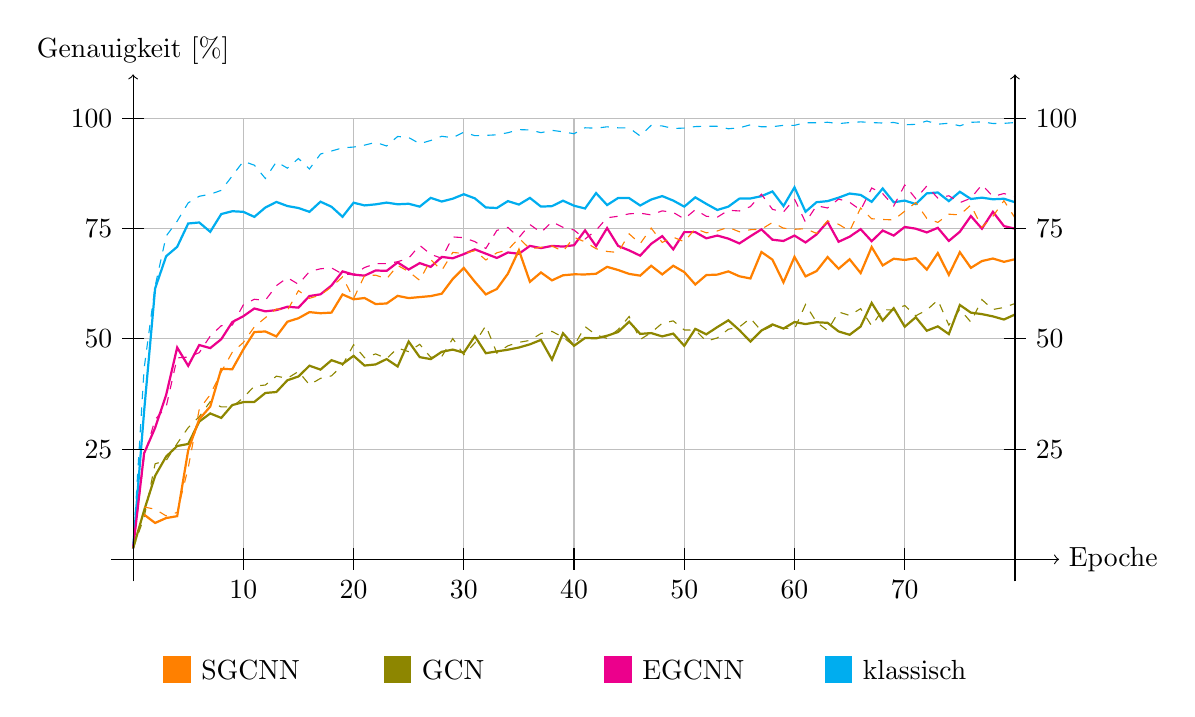
\begin{tikzpicture}[scale=1.4]
  \draw[color=lightgray] (0, 0) grid (8, 4);

  \tikzstyle{klassisch}=[color=cyan]
  \tikzstyle{egcnn}=[color=magenta]
  \tikzstyle{sgcnn}=[color=orange]
  \tikzstyle{gcn}=[color=olive]
  \tikzstyle{fillklassisch}=[fill=cyan]
  \tikzstyle{fillegcnn}=[fill=magenta]
  \tikzstyle{fillsgcnn}=[fill=orange]
  \tikzstyle{fillgcn}=[fill=olive]

  \draw[klassisch, dashed] (0, 0.1) -- (0.1, 1.7312) -- (0.2, 2.4792) -- (0.3, 2.933) -- (0.4, 3.0682) -- (0.5, 3.2344) -- (0.6, 3.2938) -- (0.7, 3.3125) -- (0.8, 3.3477) -- (0.9, 3.4792) -- (1.0, 3.6111) -- (1.1, 3.5759) -- (1.2, 3.4554) -- (1.3, 3.6066) -- (1.4, 3.5491) -- (1.5, 3.6364) -- (1.6, 3.5417) -- (1.7, 3.6771) -- (1.8, 3.7045) -- (1.9, 3.733) -- (2.0, 3.7404) -- (2.1, 3.7578) -- (2.2, 3.7831) -- (2.3, 3.75) -- (2.4, 3.8365) -- (2.5, 3.8269) -- (2.6, 3.7708) -- (2.7, 3.8) -- (2.8, 3.8382) -- (2.9, 3.825) -- (3.0, 3.875) -- (3.1, 3.8438) -- (3.2, 3.8462) -- (3.3, 3.8516) -- (3.4, 3.8705) -- (3.5, 3.8984) -- (3.6, 3.8958) -- (3.7, 3.8708) -- (3.8, 3.892) -- (3.9, 3.8787) -- (4.0, 3.8611) -- (4.1, 3.9152) -- (4.2, 3.9115) -- (4.3, 3.9241) -- (4.4, 3.9148) -- (4.5, 3.9141) -- (4.6, 3.8409) -- (4.7, 3.9375) -- (4.8, 3.9318) -- (4.9, 3.9087) -- (5.0, 3.9125) -- (5.1, 3.9261) -- (5.2, 3.9292) -- (5.3, 3.9286) -- (5.4, 3.9062) -- (5.5, 3.9148) -- (5.6, 3.9423) -- (5.7, 3.9241) -- (5.8, 3.925) -- (5.9, 3.9375) -- (6.0, 3.9375) -- (6.1, 3.9615) -- (6.2, 3.9605) -- (6.3, 3.9653) -- (6.4, 3.9531) -- (6.5, 3.9625) -- (6.6, 3.9688) -- (6.7, 3.9625) -- (6.8, 3.9583) -- (6.9, 3.9635) -- (7.0, 3.9423) -- (7.1, 3.9464) -- (7.2, 3.9766) -- (7.3, 3.9479) -- (7.4, 3.9562) -- (7.5, 3.933) -- (7.6, 3.9648) -- (7.7, 3.9688) -- (7.8, 3.9542) -- (7.9, 3.9554) -- (8.0, 3.9625);

  \draw[klassisch, thick] (0, 0.1) -- (0.1, 1.3438) -- (0.2, 2.4583) -- (0.3, 2.75) -- (0.4, 2.8352) -- (0.5, 3.0469) -- (0.6, 3.0562) -- (0.7, 2.9716) -- (0.8, 3.1328) -- (0.9, 3.1583) -- (1.0, 3.1528) -- (1.1, 3.1071) -- (1.2, 3.192) -- (1.3, 3.2426) -- (1.4, 3.2054) -- (1.5, 3.1875) -- (1.6, 3.1528) -- (1.7, 3.2448) -- (1.8, 3.1989) -- (1.9, 3.108) -- (2.0, 3.2356) -- (2.1, 3.2109) -- (2.2, 3.2206) -- (2.3, 3.2366) -- (2.4, 3.2212) -- (2.5, 3.226) -- (2.6, 3.2) -- (2.7, 3.2792) -- (2.8, 3.2463) -- (2.9, 3.2719) -- (3.0, 3.3125) -- (3.1, 3.275) -- (3.2, 3.1923) -- (3.3, 3.1875) -- (3.4, 3.25) -- (3.5, 3.2188) -- (3.6, 3.2792) -- (3.7, 3.2) -- (3.8, 3.2045) -- (3.9, 3.2537) -- (4.0, 3.2083) -- (4.1, 3.183) -- (4.2, 3.3229) -- (4.3, 3.2143) -- (4.4, 3.2784) -- (4.5, 3.2773) -- (4.6, 3.2102) -- (4.7, 3.2644) -- (4.8, 3.2955) -- (4.9, 3.2548) -- (5.0, 3.2) -- (5.1, 3.2841) -- (5.2, 3.225) -- (5.3, 3.1696) -- (5.4, 3.2) -- (5.5, 3.2727) -- (5.6, 3.274) -- (5.7, 3.2946) -- (5.8, 3.3375) -- (5.9, 3.2054) -- (6.0, 3.375) -- (6.1, 3.1538) -- (6.2, 3.2401) -- (6.3, 3.25) -- (6.4, 3.2812) -- (6.5, 3.3188) -- (6.6, 3.3062) -- (6.7, 3.2437) -- (6.8, 3.3646) -- (6.9, 3.2396) -- (7.0, 3.2548) -- (7.1, 3.2232) -- (7.2, 3.3203) -- (7.3, 3.3281) -- (7.4, 3.25) -- (7.5, 3.3348) -- (7.6, 3.2695) -- (7.7, 3.2812) -- (7.8, 3.2667) -- (7.9, 3.2715) -- (8.0, 3.2396);

  \draw[egcnn, thick] (0, 0.1) -- (0.1, 0.9625) -- (0.2, 1.1938) -- (0.3, 1.4922) -- (0.4, 1.9219) -- (0.5, 1.7557) -- (0.6, 1.9444) -- (0.7, 1.9167) -- (0.8, 1.9973) -- (0.9, 2.1528) -- (1.0, 2.2059) -- (1.1, 2.276) -- (1.2, 2.25) -- (1.3, 2.2614) -- (1.4, 2.2917) -- (1.5, 2.2837) -- (1.6, 2.3889) -- (1.7, 2.4044) -- (1.8, 2.4844) -- (1.9, 2.6125) -- (2.0, 2.5833) -- (2.1, 2.5739) -- (2.2, 2.6208) -- (2.3, 2.6172) -- (2.4, 2.6938) -- (2.5, 2.6295) -- (2.6, 2.6875) -- (2.7, 2.6534) -- (2.8, 2.7437) -- (2.9, 2.7313) -- (3.0, 2.7692) -- (3.1, 2.8125) -- (3.2, 2.7734) -- (3.3, 2.7344) -- (3.4, 2.7841) -- (3.5, 2.7723) -- (3.6, 2.8438) -- (3.7, 2.8239) -- (3.8, 2.8438) -- (3.9, 2.8375) -- (4.0, 2.85) -- (4.1, 2.9844) -- (4.2, 2.8413) -- (4.3, 3.0052) -- (4.4, 2.8438) -- (4.5, 2.8029) -- (4.6, 2.7552) -- (4.7, 2.8625) -- (4.8, 2.9323) -- (4.9, 2.8125) -- (5.0, 2.9688) -- (5.1, 2.9688) -- (5.2, 2.9125) -- (5.3, 2.9375) -- (5.4, 2.9097) -- (5.5, 2.8661) -- (5.6, 2.9312) -- (5.7, 2.9937) -- (5.8, 2.9) -- (5.9, 2.8884) -- (6.0, 2.9375) -- (6.1, 2.875) -- (6.2, 2.9479) -- (6.3, 3.0625) -- (6.4, 2.8813) -- (6.5, 2.9271) -- (6.6, 2.9952) -- (6.7, 2.8864) -- (6.8, 2.983) -- (6.9, 2.9375) -- (7.0, 3.0156) -- (7.1, 3.0) -- (7.2, 2.9659) -- (7.3, 3.0078) -- (7.4, 2.8889) -- (7.5, 2.9722) -- (7.6, 3.1146) -- (7.7, 3.0) -- (7.8, 3.1528) -- (7.9, 3.0234) -- (8.0, 3.0);

  \draw[egcnn, dashed] (0, 0.1) -- (0.1, 0.9313) -- (0.2, 1.2688) -- (0.3, 1.3828) -- (0.4, 1.8281) -- (0.5, 1.8352) -- (0.6, 1.875) -- (0.7, 2.026) -- (0.8, 2.1196) -- (0.9, 2.125) -- (1.0, 2.3088) -- (1.1, 2.3594) -- (1.2, 2.35) -- (1.3, 2.483) -- (1.4, 2.5556) -- (1.5, 2.4952) -- (1.6, 2.6111) -- (1.7, 2.636) -- (1.8, 2.6445) -- (1.9, 2.5875) -- (2.0, 2.5833) -- (2.1, 2.6477) -- (2.2, 2.6833) -- (2.3, 2.6836) -- (2.4, 2.7) -- (2.5, 2.7321) -- (2.6, 2.849) -- (2.7, 2.767) -- (2.8, 2.7313) -- (2.9, 2.925) -- (3.0, 2.9183) -- (3.1, 2.8828) -- (3.2, 2.8203) -- (3.3, 2.9844) -- (3.4, 3.0114) -- (3.5, 2.9196) -- (3.6, 3.0375) -- (3.7, 2.9659) -- (3.8, 3.0625) -- (3.9, 3.0125) -- (4.0, 2.9875) -- (4.1, 2.9062) -- (4.2, 2.9856) -- (4.3, 3.099) -- (4.4, 3.1125) -- (4.5, 3.1346) -- (4.6, 3.1406) -- (4.7, 3.125) -- (4.8, 3.1615) -- (4.9, 3.1477) -- (5.0, 3.0885) -- (5.1, 3.1719) -- (5.2, 3.1125) -- (5.3, 3.1042) -- (5.4, 3.1667) -- (5.5, 3.1607) -- (5.6, 3.2) -- (5.7, 3.3125) -- (5.8, 3.175) -- (5.9, 3.1518) -- (6.0, 3.2692) -- (6.1, 3.0583) -- (6.2, 3.2083) -- (6.3, 3.1875) -- (6.4, 3.2687) -- (6.5, 3.2396) -- (6.6, 3.1683) -- (6.7, 3.3693) -- (6.8, 3.3182) -- (6.9, 3.2062) -- (7.0, 3.3958) -- (7.1, 3.2723) -- (7.2, 3.3864) -- (7.3, 3.2773) -- (7.4, 3.2986) -- (7.5, 3.2361) -- (7.6, 3.276) -- (7.7, 3.399) -- (7.8, 3.2917) -- (7.9, 3.3188) -- (8.0, 3.2891);

  \draw[gcn, dashed] (0, 0.1) -- (0.1, 0.3812) -- (0.2, 0.8672) -- (0.3, 0.8973) -- (0.4, 1.0511) -- (0.5, 1.1953) -- (0.6, 1.2937) -- (0.7, 1.4318) -- (0.8, 1.3833) -- (0.9, 1.3833) -- (1.0, 1.4669) -- (1.1, 1.5714) -- (1.2, 1.5817) -- (1.3, 1.6618) -- (1.4, 1.6429) -- (1.5, 1.7045) -- (1.6, 1.5833) -- (1.7, 1.642) -- (1.8, 1.6648) -- (1.9, 1.7614) -- (2.0, 1.9471) -- (2.1, 1.8292) -- (2.2, 1.864) -- (2.3, 1.8214) -- (2.4, 1.9167) -- (2.5, 1.8846) -- (2.6, 1.9509) -- (2.7, 1.8333) -- (2.8, 1.8398) -- (2.9, 2.0031) -- (3.0, 1.8562) -- (3.1, 1.9625) -- (3.2, 2.1202) -- (3.3, 1.8711) -- (3.4, 1.9375) -- (3.5, 1.9688) -- (3.6, 1.9866) -- (3.7, 2.0491) -- (3.8, 2.0682) -- (3.9, 2.0147) -- (4.0, 1.9375) -- (4.1, 2.1116) -- (4.2, 2.0365) -- (4.3, 2.0048) -- (4.4, 2.0852) -- (4.5, 2.2031) -- (4.6, 1.9943) -- (4.7, 2.0577) -- (4.8, 2.142) -- (4.9, 2.1635) -- (5.0, 2.0812) -- (5.1, 2.0795) -- (5.2, 1.9792) -- (5.3, 2.0089) -- (5.4, 2.0875) -- (5.5, 2.108) -- (5.6, 2.1875) -- (5.7, 2.0714) -- (5.8, 2.1187) -- (5.9, 2.0982) -- (6.0, 2.0909) -- (6.1, 2.3125) -- (6.2, 2.1513) -- (6.3, 2.0764) -- (6.4, 2.2448) -- (6.5, 2.2125) -- (6.6, 2.275) -- (6.7, 2.1181) -- (6.8, 2.2656) -- (6.9, 2.2614) -- (7.0, 2.3029) -- (7.1, 2.2098) -- (7.2, 2.2617) -- (7.3, 2.3523) -- (7.4, 2.125) -- (7.5, 2.2692) -- (7.6, 2.1523) -- (7.7, 2.3563) -- (7.8, 2.2667) -- (7.9, 2.2852) -- (8.0, 2.3210);

  \draw[gcn, thick] (0, 0.1) -- (0.1, 0.4437) -- (0.2, 0.7578) -- (0.3, 0.933) -- (0.4, 1.0284) -- (0.5, 1.0469) -- (0.6, 1.25) -- (0.7, 1.3239) -- (0.8, 1.2833) -- (0.9, 1.4) -- (1.0, 1.4265) -- (1.1, 1.4286) -- (1.2, 1.5096) -- (1.3, 1.5184) -- (1.4, 1.625) -- (1.5, 1.6591) -- (1.6, 1.7569) -- (1.7, 1.7216) -- (1.8, 1.8068) -- (1.9, 1.7727) -- (2.0, 1.8462) -- (2.1, 1.7583) -- (2.2, 1.7684) -- (2.3, 1.817) -- (2.4, 1.75) -- (2.5, 1.976) -- (2.6, 1.8348) -- (2.7, 1.8167) -- (2.8, 1.8828) -- (2.9, 1.9031) -- (3.0, 1.875) -- (3.1, 2.025) -- (3.2, 1.8702) -- (3.3, 1.8867) -- (3.4, 1.9018) -- (3.5, 1.9219) -- (3.6, 1.9509) -- (3.7, 1.9911) -- (3.8, 1.8125) -- (3.9, 2.0515) -- (4.0, 1.9375) -- (4.1, 2.0089) -- (4.2, 2.0052) -- (4.3, 2.0288) -- (4.4, 2.0625) -- (4.5, 2.1562) -- (4.6, 2.0455) -- (4.7, 2.0529) -- (4.8, 2.0227) -- (4.9, 2.0481) -- (5.0, 1.9375) -- (5.1, 2.0909) -- (5.2, 2.0417) -- (5.3, 2.1071) -- (5.4, 2.1688) -- (5.5, 2.0795) -- (5.6, 1.976) -- (5.7, 2.0759) -- (5.8, 2.1313) -- (5.9, 2.0938) -- (6.0, 2.1534) -- (6.1, 2.1346) -- (6.2, 2.1513) -- (6.3, 2.1458) -- (6.4, 2.0677) -- (6.5, 2.0375) -- (6.6, 2.1125) -- (6.7, 2.3264) -- (6.8, 2.1667) -- (6.9, 2.2784) -- (7.0, 2.1106) -- (7.1, 2.1964) -- (7.2, 2.0742) -- (7.3, 2.1136) -- (7.4, 2.0438) -- (7.5, 2.3077) -- (7.6, 2.2383) -- (7.7, 2.225) -- (7.8, 2.2042) -- (7.9, 2.1758) -- (8.0, 2.2214);

  \draw[sgcnn, thick] (0.1, 0.4062) -- (0.2, 0.3304) -- (0.3, 0.375) -- (0.4, 0.392) -- (0.5, 0.9911) -- (0.6, 1.2708) -- (0.7, 1.3864) -- (0.8, 1.7277) -- (0.9, 1.725) -- (1.0, 1.9044) -- (1.1, 2.0625) -- (1.2, 2.0673) -- (1.3, 2.0223) -- (1.4, 2.1562) -- (1.5, 2.1875) -- (1.6, 2.2431) -- (1.7, 2.233) -- (1.8, 2.2386) -- (1.9, 2.4034) -- (2.0, 2.3594) -- (2.1, 2.3708) -- (2.2, 2.3164) -- (2.3, 2.3214) -- (2.4, 2.3906) -- (2.5, 2.3702) -- (2.6, 2.3795) -- (2.7, 2.3884) -- (2.8, 2.4102) -- (2.9, 2.5438) -- (3.0, 2.6437) -- (3.1, 2.5187) -- (3.2, 2.4038) -- (3.3, 2.4531) -- (3.4, 2.5913) -- (3.5, 2.8047) -- (3.6, 2.5179) -- (3.7, 2.6027) -- (3.8, 2.5312) -- (3.9, 2.5772) -- (4.0, 2.5859) -- (4.1, 2.5848) -- (4.2, 2.5909) -- (4.3, 2.6538) -- (4.4, 2.625) -- (4.5, 2.5898) -- (4.6, 2.5739) -- (4.7, 2.6635) -- (4.8, 2.5852) -- (4.9, 2.6635) -- (5.0, 2.6063) -- (5.1, 2.4937) -- (5.2, 2.5792) -- (5.3, 2.5833) -- (5.4, 2.6125) -- (5.5, 2.5682) -- (5.6, 2.5481) -- (5.7, 2.7885) -- (5.8, 2.7188) -- (5.9, 2.5134) -- (6.0, 2.7443) -- (6.1, 2.5673) -- (6.2, 2.6151) -- (6.3, 2.7422) -- (6.4, 2.6364) -- (6.5, 2.7222) -- (6.6, 2.5972) -- (6.7, 2.8333) -- (6.8, 2.6667) -- (6.9, 2.7273) -- (7.0, 2.7163) -- (7.1, 2.7321) -- (7.2, 2.6289) -- (7.3, 2.7784) -- (7.4, 2.5812) -- (7.5, 2.7865) -- (7.6, 2.6445) -- (7.7, 2.7062) -- (7.8, 2.7292) -- (7.9, 2.6992) -- (8.0, 2.7227);

  \draw[sgcnn, dashed] (0.1, 0.475) -- (0.2, 0.4554) -- (0.3, 0.3942) -- (0.4, 0.4261) -- (0.5, 0.8304) -- (0.6, 1.3611) -- (0.7, 1.4943) -- (0.8, 1.7009) -- (0.9, 1.8792) -- (1.0, 1.9669) -- (1.1, 2.1094) -- (1.2, 2.1923) -- (1.3, 2.2723) -- (1.4, 2.2589) -- (1.5, 2.4375) -- (1.6, 2.3681) -- (1.7, 2.3977) -- (1.8, 2.4716) -- (1.9, 2.5625) -- (2.0, 2.3646) -- (2.1, 2.575) -- (2.2, 2.5781) -- (2.3, 2.5446) -- (2.4, 2.6667) -- (2.5, 2.6106) -- (2.6, 2.5312) -- (2.7, 2.7188) -- (2.8, 2.6211) -- (2.9, 2.7844) -- (3.0, 2.775) -- (3.1, 2.8) -- (3.2, 2.7163) -- (3.3, 2.7812) -- (3.4, 2.8077) -- (3.5, 2.9141) -- (3.6, 2.817) -- (3.7, 2.8304) -- (3.8, 2.8438) -- (3.9, 2.7941) -- (4.0, 2.9219) -- (4.1, 2.8795) -- (4.2, 2.8182) -- (4.3, 2.7933) -- (4.4, 2.7841) -- (4.5, 2.9531) -- (4.6, 2.8636) -- (4.7, 3.0048) -- (4.8, 2.875) -- (4.9, 2.9231) -- (5.0, 2.8813) -- (5.1, 3.0) -- (5.2, 2.9625) -- (5.3, 2.9792) -- (5.4, 3.0125) -- (5.5, 2.9716) -- (5.6, 2.9904) -- (5.7, 2.9952) -- (5.8, 3.0562) -- (5.9, 3.0045) -- (6.0, 2.9943) -- (6.1, 3.0) -- (6.2, 2.9572) -- (6.3, 3.0703) -- (6.4, 3.0398) -- (6.5, 2.9792) -- (6.6, 3.1875) -- (6.7, 3.0903) -- (6.8, 3.0833) -- (6.9, 3.0795) -- (7.0, 3.1587) -- (7.1, 3.2366) -- (7.2, 3.0938) -- (7.3, 3.0568) -- (7.4, 3.1313) -- (7.5, 3.125) -- (7.6, 3.2148) -- (7.7, 3.0125) -- (7.8, 3.1125) -- (7.9, 3.2539) -- (8.0, 3.0977);


  \draw (0.1, 4) -- (-0.1, 4) node[left] {$100$};
  \draw (0.1, 3) -- (-0.1, 3) node[left] {$75$};
  \draw (0.1, 2) -- (-0.1, 2) node[left] {$50$};
  \draw (0.1, 1) -- (-0.1, 1) node[left] {$25$};

  \draw (7.9, 4) -- (8.1, 4) node[right] {$100$};
  \draw (7.9, 3) -- (8.1, 3) node[right] {$75$};
  \draw (7.9, 2) -- (8.1, 2) node[right] {$50$};
  \draw (7.9, 1) -- (8.1, 1) node[right] {$25$};

  \draw (1, 0.1) -- (1, -0.1)  node[below] {$10$};
  \draw (2, 0.1) -- (2, -0.1)  node[below] {$20$};
  \draw (3, 0.1) -- (3, -0.1)  node[below] {$30$};
  \draw (4, 0.1) -- (4, -0.1)  node[below] {$40$};
  \draw (5, 0.1) -- (5, -0.1)  node[below] {$50$};
  \draw (6, 0.1) -- (6, -0.1)  node[below] {$60$};
  \draw (7, 0.1) -- (7, -0.1)  node[below] {$70$};

  \draw[->] (-0.2, 0)    -- (8.4, 0)   node[right] {Epoche};
  \draw[->] (0,    -0.2) -- (0,   4.4) node[above] {Genauigkeit [\%]};
  \draw[->] (8,    -0.2) -- (8,   4.4);

  \tikzstyle{node}=[rectangle, minimum width=10pt, minimum height=10pt, inner sep=0pt]
  \node[node, fillsgcnn,     label=right:\gls{SGCNN}] (1) at (0.4, -1) {};
  \node[node, fillgcn,       label=right:\gls{GCN}]   (2) at (2.4, -1) {};
  \node[node, fillegcnn,     label=right:\gls{EGCNN}] (3) at (4.4, -1) {};
  \node[node, fillklassisch, label=right:klassisch]   (4) at (6.4, -1) {};

\end{tikzpicture}
\caption[\gls{Cifar}-10 Genauigkeitsverlauf über Quickshift]{Genauigkeitsverlauf eines Trainings auf dem \gls{Cifar}-10 Datensatz der spektralen Ansätze auf Graphen im zweidimensionalen euklidischen Raum, welche über Quickshift generiert wurden, sowie dem klassischen Ansatz auf Bildern.
Die gestrichelten Linien zeigen die Genauigkeiten des Trainingsdatensatzes in Abhängigkeit der Epochen, wohingegen die durchgezogenen Linien sich auf den Validierungsdatensatz beziehen.}
\label{fig:cifar_10_train}
\end{figure}


% Postprocessing weitaus besser als preprocessing!

LearningRate: 0.001
LearningRateDecay: Alle 5000 Steps um 0.96
BatchSize: 64
WeightDecay in FC256 und FC128: 0.004
Dropout vor letztem: 0.5
jeweils 65k Steps (entspricht ungefähr 75 Epochen)
65k steps trainiert: vereinheitlichen wir zu 60k

\begin{table}[t]
\centering
\resizebox{\textwidth}{!}{%
\begin{tabular}{lclrrr}
  \toprule
  Ansatz & \ma{W} & Architektur & \multicolumn{2}{c}{Genauigkeit [\%]}\\
  \cmidrule{4-5}
   & & & \gls{SLIC} & \acs{QS}\\
  \midrule
  \acs{SGCNN} & 9 & C64-P2-C128-P2-C256-P2-C512-Avg-FC256-FC128 & & 67.748\\
  \acs{GCN} & 1 & C64-C64-P2-C128-P2-C256-P2-C512-Avg-FC256-FC128 & 54.497 & 53.606\\
  \acs{EGCNN} & 9 & C64-C64-P2-C128-P2-C256-P2-C512-Avg-FC256-FC128 & 74.218 & 75.230\\
  \midrule
  klassisch & $3 \times 3$ & C64-C64-P4-C128-P4-C256-P4-FC256-FC128 & \multicolumn{2}{c}{82.061} \\
  \bottomrule
\end{tabular}}
\caption[Testgenauigkeiten der \gls{Cifar}-10 Superpixelrepräsentationen]{65k steps}
\label{tab:train_cifar_10}
\end{table}

\paragraph{\gls{Pascal}}

\begin{table}[t]
\centering
\resizebox{\textwidth}{!}{%
\begin{tabular}{lclrrr}
  \toprule
  Ansatz & \ma{W} & Architektur & \multicolumn{2}{c}{Genauigkeit [\%]}\\
  \cmidrule{4-5}
   & & & \gls{SLIC} & \acs{QS}\\
  \midrule
  \acs{EGCNN} & 9 & &\\
  \midrule
  klassisch & — & SqueezeNet 1.1 & \multicolumn{2}{c}{54.731} \\
  \bottomrule
\end{tabular}}
\caption[Testgenauigkeiten der \gls{Pascal} Superpixelrepräsentationen]{50k Steps}
\label{tab:train_pascal}
\end{table}

PascalVOC Squeeze einheitliche Größe von $224 \times 224$.
Squeeze vorstellen
insbesondere nur Vorverarbeitung vorm Training (aufgrund Laufzeiten)

% Alle Faltungen wurden dabei mit einer Partitionsgröße von $8$ bei $K=0$ und $K=1$ implementiert, um ein \gls{CNN} mit einem $3 \times 3$ Filter zu simulieren.
% Es erscheint jedoch vorstellbar die Filtergröße bei größerer lokaler Kontrollierbarkeit, \dhe{} $K > 1$, weiter zu reduzieren und die Gefahr des Overfittings damit aufgrund der kleineren Anzahl an Trainingsparametern einzuschränken.


Alle Faltungen wurden dabei mit einer Partitionsgröße von $8$ bei $K=0$ und $K=1$ implementiert, um ein \gls{CNN} mit einem $3 \times 3$ Filter zu simulieren.
Es erscheint jedoch vorstellbar die Filtergröße bei größerer lokaler Kontrollierbarkeit, \dhe{} $K > 1$, weiter zu reduzieren und die Gefahr des Overfittings damit auf Grund der kleineren Anzahl an Trainingsparametern einzuschränken.

\section{Laufzeitanalyse}
\label{laufzeitanalyse}

% Das Training des neuronalen Netzes und der Betrieb des in Kapitel 3.4 vorgestell- ten Systems erfolgte auf einem Intel R CoreTM i5 Prozessor mit 3,2 Ghz, 16GB Ar- beitsspeicher und einer Nvidia R GeForceTM 980GTX Grafikkarte.
Rechnerhardware vorstellen

Laufzeitvergleich Slic Quickshift
Laufzeitvergleich Normales CNN und die entsprechenden Graphimplementierungen
Laufzeitvergleich CPU GPU

Laufzeitvergleich Preprocessing / ohne (+ Verhältnis Faltung / Preprocessing)

Cifar-10 Quickshift: Ohne Preprocessing: 0.03s
mit: 0.29s (Batch-Size 64)

\begin{figure}[t]
\centering
  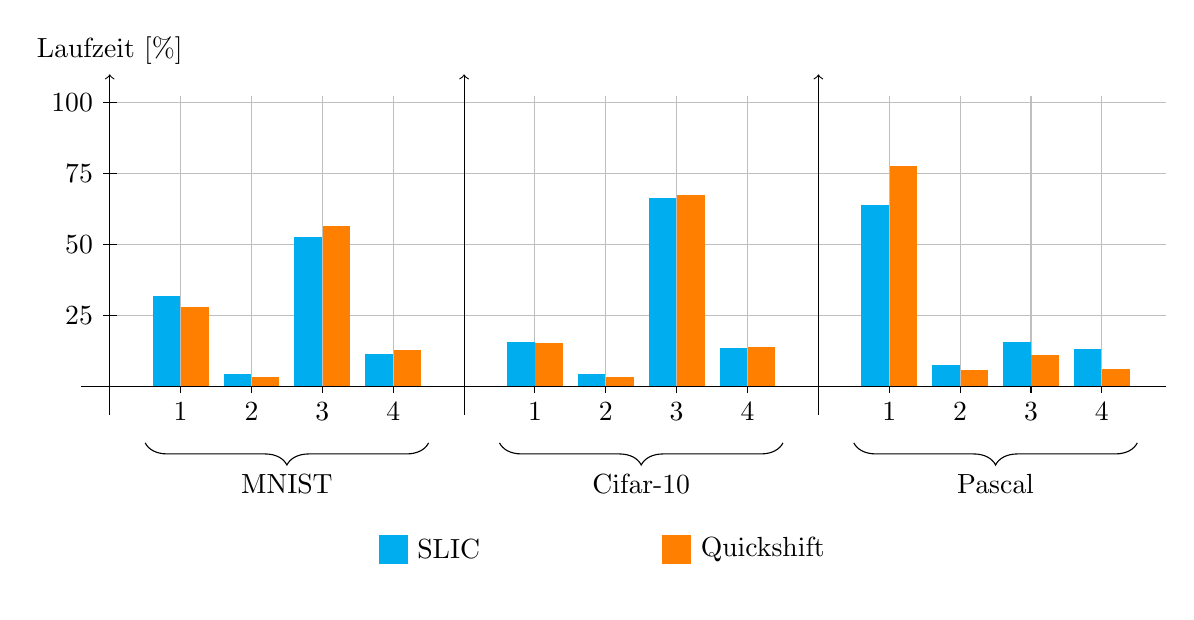
\begin{tikzpicture}[scale=0.9]
  \tikzstyle{slic}=[color=cyan, fill=cyan]
  \tikzstyle{quickshift}=[color=orange, fill=orange]

  \fill[white] (0, -2.9) rectangle (1, -1) node {};  % Abstand nach unten

  \draw[color=lightgray] (-0.1, -0.1) grid (14.9, 4.1);

  \draw[] (-0.4, 0) -- (14.9, 0);
  \draw[->] (0, -0.4) -- (0, 4.4) node[above] {Laufzeit [\%]};
  \draw[->] (5, -0.4) -- (5, 4.4);
  \draw[->] (10, -0.4) -- (10, 4.4);

  \draw (0.1, 1) -- (-0.1, 1) node[left] {$25$};
  \draw (0.1, 2) -- (-0.1, 2) node[left] {$50$};
  \draw (0.1, 3) -- (-0.1, 3) node[left] {$75$};
  \draw (0.1, 4) -- (-0.1, 4) node[left] {$100$};

  \draw[slic,       line width=0.35cm] (0.8, 0) -- (0.8, 4*0.3179);
  \draw[quickshift, line width=0.35cm] (1.2, 0) -- (1.2, 4*0.2792);
  \draw (1, 0) -- (1, -0.1) node[below] {$1$};

  \draw[slic,       line width=0.35cm] (1.8, 0) -- (1.8, 4*0.0445);
  \draw[quickshift, line width=0.35cm] (2.2, 0) -- (2.2, 4*0.0313);
  \draw (2, 0) -- (2, -0.1) node[below] {$2$};

  \draw[slic,       line width=0.35cm] (2.8, 0) -- (2.8, 4*0.5255);
  \draw[quickshift, line width=0.35cm] (3.2, 0) -- (3.2, 4*0.5633);
  \draw (3, 0) -- (3, -0.1) node[below] {$3$};

  \draw[slic,       line width=0.35cm] (3.8, 0) -- (3.8, 4*0.1120);
  \draw[quickshift, line width=0.35cm] (4.2, 0) -- (4.2, 4*0.1263);
  \draw (4, 0) -- (4, -0.1) node[below] {$4$};

  \draw [decoration={brace,mirror,amplitude=8pt},decorate] (0.5,-0.8) -- node[below=8pt] {\gls{MNIST}} (4.5,-0.8);

  \draw[slic,       line width=0.35cm] (5.8, 0) -- (5.8, 4*0.1543);
  \draw[quickshift, line width=0.35cm] (6.2, 0) -- (6.2, 4*0.1538);
  \draw (6, 0) -- (6, -0.1) node[below] {$1$};

  \draw[slic,       line width=0.35cm] (6.8, 0) -- (6.8, 4*0.0446);
  \draw[quickshift, line width=0.35cm] (7.2, 0) -- (7.2, 4*0.0325);
  \draw (7, 0) -- (7, -0.1) node[below] {$2$};

  \draw[slic,       line width=0.35cm] (7.8, 0) -- (7.8, 4*0.6653);
  \draw[quickshift, line width=0.35cm] (8.2, 0) -- (8.2, 4*0.6759);
  \draw (8, 0) -- (8, -0.1) node[below] {$3$};

  \draw[slic,       line width=0.35cm] (8.8, 0) -- (8.8, 4*0.1358);
  \draw[quickshift, line width=0.35cm] (9.2, 0) -- (9.2, 4*0.1378);
  \draw (9, 0) -- (9, -0.1) node[below] {$4$};

    \draw [decoration={brace,mirror,amplitude=8pt},decorate] (5.5,-0.8) -- node[below=8pt] {\gls{Cifar}-10} (9.5,-0.8);

  \draw[slic,       line width=0.35cm] (10.8, 0) -- (10.8, 4*0.6384);
  \draw[quickshift, line width=0.35cm] (11.2, 0) -- (11.2, 4*0.7750);
  \draw (11, 0) -- (11, -0.1) node[below] {$1$};

  \draw[slic,       line width=0.35cm] (11.8, 0) -- (11.8, 4*0.0741);
  \draw[quickshift, line width=0.35cm] (12.2, 0) -- (12.2, 4*0.0559);
  \draw (12, 0) -- (12, -0.1) node[below] {$2$};

  \draw[slic,       line width=0.35cm] (12.8, 0) -- (12.8, 4*0.1573);
  \draw[quickshift, line width=0.35cm] (13.2, 0) -- (13.2, 4*0.1100);
  \draw (13, 0) -- (13, -0.1) node[below] {$3$};

  \draw[slic,       line width=0.35cm] (13.8, 0) -- (13.8, 4*0.1302);
  \draw[quickshift, line width=0.35cm] (14.2, 0) -- (14.2, 4*0.0591);
  \draw (14, 0) -- (14, -0.1) node[below] {$4$};

  \draw [decoration={brace,mirror,amplitude=8pt},decorate] (10.5,-0.8) -- node[below=8pt] {\gls{Pascal}} (14.5,-0.8);

  \tikzstyle{node}=[rectangle,draw, minimum width=10pt, minimum height=10pt, inner sep=0pt]
  \node[node, slic,       label=right:\gls{SLIC}] (1) at (4, -2.3) {};
  \node[node, quickshift, label=right:Quickshift] (2) at (8, -2.3) {};
\end{tikzpicture}

\begin{tabular}{ll}
  \toprule
  1. Segmentierung & 2. Adjazenzbestimmung\\
  3. Graphvergröberung (4 Ebenen) & 4. Merkmalsextraktion\\
  \bottomrule
\end{tabular}

\caption[Laufzeitverteilung der spektralen Vorverarbeitungsschritte]{Laufzeitverteilung der einzelnen spektralen Vorverarbeitungsschritte für alle Datensätze und Superpixelalgorithmen.
Wohingegen für \gls{MNIST} und \gls{Cifar}-10 die Graphvergröberung die längste Berechnungsdauer in Anspruch nimmt, zeigt sich dagegegen für größere Datensätze wie \gls{Pascal} die Segmentierung als Flaschenhals der Vorverarbeitung.}
\label{fig:laufzeit_spektral_pipeline}
\end{figure}


\paragraph{Vergleich \bzgl{} vorhandener Implementierungen}
\label{vergleich_laufzeit}

\begin{figure}[t]
\centering
  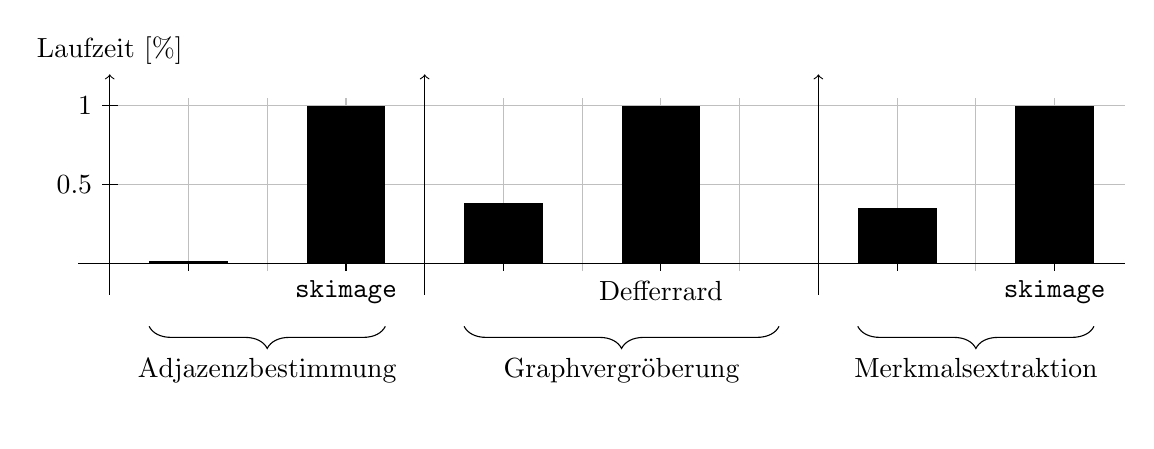
\begin{tikzpicture}[]
  \fill[white] (0, -2) rectangle (1, -1) node {};  % Abstand nach unten

  \draw[color=lightgray] (-0.1, -0.1) grid (12.9, 2.1);

  \draw[] (-0.4, 0) -- (12.9, 0);
    \draw[->] (0, -0.4) -- (0, 2.4) node[above] {Laufzeit [\%]};
  \draw[->] (4, -0.4) -- (4, 2.4);
  \draw[->] (9, -0.4) -- (9, 2.4);

  \draw (0.1, 1) -- (-0.1, 1) node[left] {$0.5$};
  \draw (0.1, 2) -- (-0.1, 2) node[left] {$1$};

  \draw[line width=1cm] (1, 0) -- (1, 0.030153);
  \draw[line width=1cm] (3, 0) -- (3, 2);
  \draw (1, 0) -- (1, -0.1);
  \draw (3, 0) -- (3, -0.1) node[below] {\texttt{skimage}};
  \draw [decoration={brace,mirror,amplitude=8pt},decorate] (0.5,-0.8) -- node[below=8pt] {Adjazenzbestimmung} (3.5,-0.8);

  \draw[line width=1cm] (5,  0) -- (5,  0.769867);
  \draw[line width=1cm] (7, 0)  -- (7, 2);
  \draw (5, 0) -- (5, -0.1);
  \draw (7, 0) -- (7, -0.1) node[below] {\citeauthor{Defferrard}};
  \draw [decoration={brace,mirror,amplitude=8pt},decorate] (4.5,-0.8) -- node[below=8pt] {Graphvergröberung} (8.5,-0.8);

  \draw[line width=1cm] (10, 0)  -- (10, 0.704036);
  \draw[line width=1cm] (12, 0) -- (12, 2);
  \draw (10, 0)  -- (10,  -0.1);
  \draw (12, 0) -- (12, -0.1) node[below] {\texttt{skimage}};
  \draw [decoration={brace,mirror,amplitude=8pt},decorate] (9.5,-0.8) -- node[below=8pt] {Merkmalsextraktion} (12.5,-0.8);

\end{tikzpicture}

\begin{tabular}{lrrr}
  \toprule
  Vorverarbeitungsschritt & vorhanden [ms] & optimiert [ms] & Gewinn [\%]\\
  \midrule
  Adjazenzbestimmung & 866 & 13 & 6535\\
  Graphvergröberung & 87 & 33 & 160\\
  Merkmalsextraktion & 144 & 50 & 184\\
  \bottomrule
\end{tabular}

  \caption[Laufzeitvergleich \bzgl{} anderer Implementierungen]{Vergleich der Laufzeiten verschiedener Vorverarbeitungsschritte \bzgl{} des Lernens auf Graphen zwischen bereits vorhandenen, quelloffenen Implementierungen (rechts) und ihrer jeweiligen optimierten Version (links) am Beispiel eines Bildes aus \gls{Pascal}:\@ (a) Adjazenzbestimmung einer Segmentierungsmaske, (b) Graphvergröberungsschritt inklusive der entsprechenden Anordung der Knoten zu binären Bäumen und (c) Merkmalsextraktion.
  In allen Bereichen konnten deutliche Laufzeitgewinne erreicht werden.}
\label{fig:laufzeit_vergleich}
\end{figure}


\section{Diskussion}
\label{diskussion}

% Patchy ist translationsinvaraint!!! sehr schnell aufgrund der nutzung des für GPU optimierten klasssischen conv2d
% kann jedoch nur eine faltungsschicht enthalten
% ein pooling, die mehrere Faltungsschichten in verschiedenen Auflösungen ermöglicht, ist aufgrund der festlegeten Knotenauswahl nicht einfach möglich.

% bei der generierung des cubes können viele Duplikate gespeichert werden (räumlich)

% Würfel ist speicherineffizient
% Eigentliche Graphstruktur geht verloren (\zB{} Distanzen der Knoten zueinander) (in gewisser weise stecken diese aber in den Formfeatures).

% Die Anordnung der Knoten zu einem Quaderform besitzt damit die Einschränkung, dass das Netz lediglich eine Faltungsschicht enthalten kann.
% Die Methode der spektralen Faltung auf Graphen umgeht diese Einschränkung.

% Würfel ist speicherineffizient

